\documentclass[11pt]{article}

\usepackage[a4paper,margin=0.92in]{geometry}
\usepackage[T1]{fontenc}
\usepackage[utf8]{inputenc}
\usepackage{lmodern}
\usepackage{microtype}
\usepackage{amsmath,amssymb,amsthm,mathtools}
\usepackage{booktabs,array}
\usepackage{graphicx}
\usepackage{enumitem}
\usepackage{xcolor}
\usepackage[hidelinks]{hyperref}

\emergencystretch=2em
\graphicspath{{../figures/}}
% Auto-generated by scripts/028_generate_pandrosion_relativity_benchmarks.py
\newcommand{\MinkFineDx}{0.01250}
\newcommand{\MinkFinePathError}{0.00500}
\newcommand{\MinkFineTauError}{6.598346e-03}
\newcommand{\MinkExactTau}{4.853864}
\newcommand{\MinkFineTau}{4.847266}
\newcommand{\NewtonFineDx}{0.00500}
\newcommand{\NewtonFineMaxError}{0.01200}
\newcommand{\NewtonFineRmsError}{0.00851}
\newcommand{\NewtonGravity}{0.350}
\newcommand{\HorizonSwitchRadius}{2.603}
\newcommand{\HorizonSwitchTime}{3.290}
\newcommand{\HorizonPGTau}{4.447376}
\newcommand{\HorizonPGTauError}{9.059420e-14}
\newcommand{\HorizonEndTime}{4.447376}


\hypersetup{
  pdftitle={Pandrosion Relativity Benchmarks},
  pdfauthor={Ivan Besevic},
  pdfsubject={Numerical finite-probe benchmarks for Pandrosion relativity},
  pdfkeywords={Pandrosion, relativity, causal graph, Newtonian limit, horizon, dynamic atlas}
}

\newtheorem{definition}{Definition}[section]
\newtheorem{proposition}[definition]{Proposition}
\newtheorem{theorem}[definition]{Theorem}
\newtheorem{conjecture}[definition]{Conjecture}
\newtheorem{remark}[definition]{Remark}

\newcommand{\R}{\mathbb R}
\newcommand{\Cset}{\mathcal C}
\newcommand{\J}{\mathcal J}
\newcommand{\T}{\mathcal T}
\newcommand{\dd}{\,\mathrm d}
\newcommand{\Oterm}{\mathcal O}
\newcommand{\norm}[1]{\left\lVert #1\right\rVert}
\DeclareMathOperator*{\argmax}{arg\,max}

\title{Pandrosion Relativity Benchmarks\\[3pt]
\large Minkowski recovery, Newtonian shadow, and horizon-safe dynamic atlases}
\author{Ivan Besevic\\Independent Mathematical Research}
\date{May 2026}

\begin{document}
\maketitle

\begin{abstract}
Paper 027 formulated Pandrosion relativity as a finite-probe version of
relativistic geodesic motion: causal candidate endpoints, a discrete
proper-time score, and dynamic atlas selection.  The present paper turns that
formulation into reproducible numerical tests.  Three benchmarks are built.
First, in \(1+1\) Minkowski space, a causal graph maximizer recovers the
straight inertial worldline and its proper time.  Second, the weak-field
order-\(c^{-2}\) Pandrosion score recovers Newton's equation; for a constant
field the selected bridge converges to the classical parabola.  Third, for
radial infall near a Schwarzschild horizon, the dynamic atlas rejects the
ill-conditioned Schwarzschild chart and switches to a regular
Painleve--Gullstrand chart before the horizon.

The experiments are intentionally conservative.  They do not claim a new
relativistic law.  The novelty is the Pandrosion organization of the
calculation: finite causal probes, proper-time maximization, weak-field
Newtonian shadow, and chart-conditioning logic are tested as one algorithmic
pipeline.  In the finest runs reported here, the Minkowski path error is
\(\MinkFinePathError\) at mesh \(\Delta x=\MinkFineDx\), the Newtonian bridge
has RMS error \(\NewtonFineRmsError\) at mesh \(\Delta x=\NewtonFineDx\), and
the horizon atlas switches to the regular chart at
\(r\simeq \HorizonSwitchRadius M\).
\end{abstract}

\paragraph{One-sentence summary.}
028 makes 027 operational: finite Pandrosion probes reproduce the inertial
line, the Newtonian parabola, and a horizon-safe chart switch in explicit
computations.

\paragraph{Is it new?}
The physical laws and many numerical ingredients are classical.  What is new
inside this Pandrosion program is the combined protocol: causal finite-slope
probe graphs, proper-time scoring, a Newtonian shadow test, and dynamic atlas
conditioning presented as one Pandrosion benchmark suite.

\paragraph{Reproducibility.}
All figures and numerical constants in this paper are generated by
\[
        \texttt{scripts/028\_generate\_pandrosion\_relativity\_benchmarks.py}.
\]

\tableofcontents

\section{Why a benchmark paper is needed}

Paper 027 gave the geometric formulation.  A formulation is not enough.  A
Pandrosion physical law should pass minimal tests:
\begin{enumerate}[label=(\roman*)]
\item in flat spacetime it must recover inertial motion;
\item in the weak-field slow-motion limit it must recover Newton's equation;
\item near a coordinate singularity it must switch charts instead of treating
the coordinate blow-up as physical.
\end{enumerate}
The three tests below are designed exactly for those checks.  They are small,
controlled, and reproducible.

\section{Benchmark 1: Minkowski causal graph}

Use \(1+1\) Minkowski spacetime with units \(c=1\):
\[
        \dd s^2=-\dd t^2+\dd x^2.
\]
For a future timelike segment \((\Delta t,\Delta x)\), the finite proper time
is
\[
        \tau(\Delta t,\Delta x)
        =
        \sqrt{\Delta t^2-\Delta x^2}.
\]
Given endpoints \((0,0)\) and \((T,X)\), the Pandrosion graph score is
\[
        \J_h(\Gamma)
        =
        \sum_{k=0}^{N-1}
        \sqrt{\Delta t_k^2-\Delta x_k^2},
        \qquad |\Delta x_k|<\Delta t_k.
\]

\begin{proposition}[Flat-space calibration]
Among future timelike broken lines from \((0,0)\) to \((T,X)\), with
\(|X|<T\), the proper-time score satisfies
\[
        \sum_k \sqrt{\Delta t_k^2-\Delta x_k^2}
        \le
        \sqrt{T^2-X^2}.
\]
Equality holds exactly when all segments have the same velocity
\(\Delta x_k/\Delta t_k=X/T\).  Thus the continuum Pandrosion score selects
the inertial line.
\end{proposition}

\begin{proof}
The statement is the reverse triangle inequality for future timelike vectors.
Equivalently, the function \(v\mapsto\sqrt{1-v^2}\) is concave on
\((-1,1)\), so Jensen's inequality gives the result after writing
\(\Delta x_k=v_k\Delta t_k\).
\end{proof}

\begin{figure}[htbp]
\centering
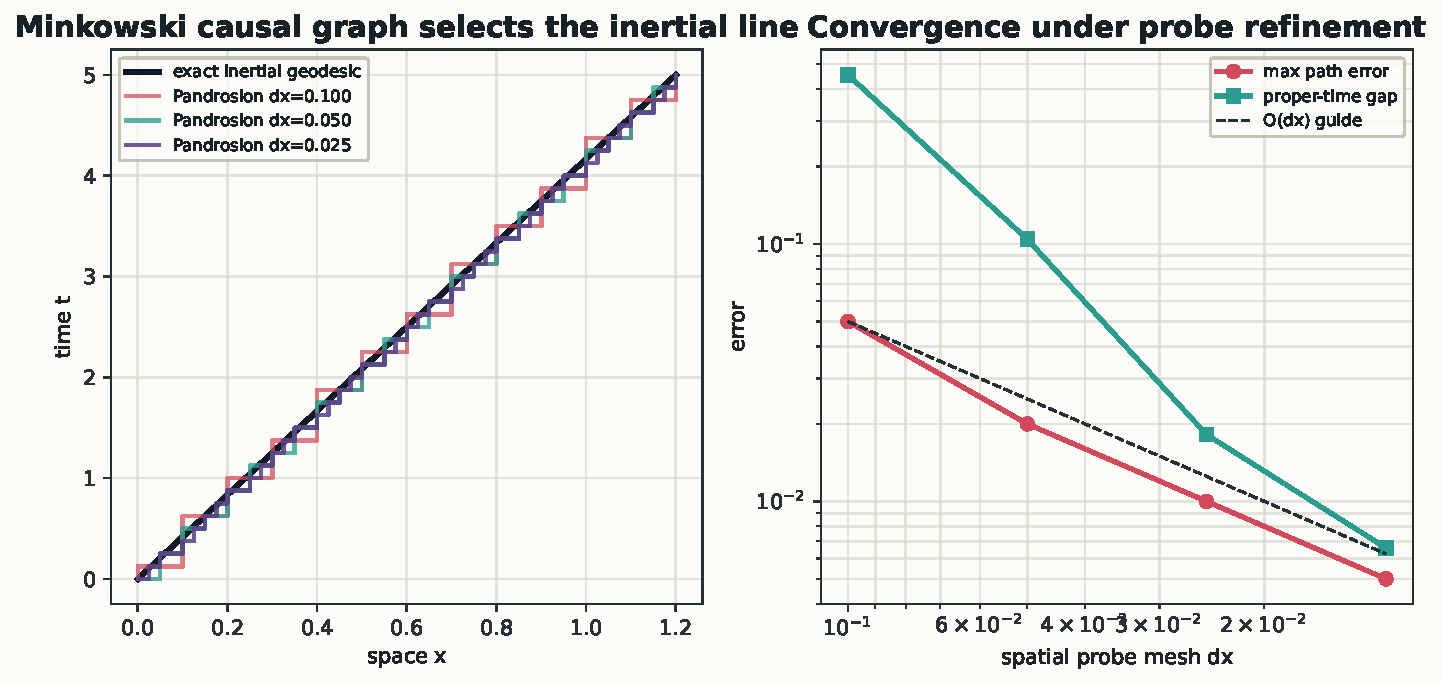
\includegraphics[width=0.96\linewidth]{028_minkowski_causal_dp.pdf}
\caption{Minkowski benchmark.  The causal graph maximizes finite proper time
between fixed endpoints.  The balanced lattice maximizer approaches the
straight inertial worldline as the spatial probe mesh is refined.}
\label{fig:minkowski}
\end{figure}

The implemented graph uses \(T=5\), \(X=1.2\), \(N=40\) time slices and
spatial meshes from \(0.1\) down to \(\MinkFineDx\).  The finest run gives
\[
        \T_{\mathrm{exact}}=\MinkExactTau,
        \qquad
        \T_h=\MinkFineTau,
        \qquad
        |\T_{\mathrm{exact}}-\T_h|=\MinkFineTauError.
\]
A vanishing tie-breaker selects the balanced representative among lattice
paths with equal leading proper-time score.  This tie-breaker is diagnostic;
the invariant leading score is the proper time above.

\section{Benchmark 2: Newtonian shadow}

Restore \(c\) and use a weak static metric
\[
        \dd s^2
        =
        -\left(1+\frac{2\Phi(x)}{c^2}\right)c^2\dd t^2
        +
        \dd x^2
        +
        \Oterm(c^{-2}\norm{\dd x}^2).
\]
For slow motion,
\[
        \dd\tau
        =
        \left[
        1+\frac{\Phi(x)}{c^2}
        -
        \frac{\dot x^2}{2c^2}
        \right]\dd t
        +
        \Oterm(c^{-4}).
\]
After dropping the constant factor, the Pandrosion weak-field score is
\[
        \J_h^{\mathrm{Newt}}(\Gamma)
        =
        \sum_k
        \Delta t
        \left[
        \Phi\!\left(\frac{x_k+x_{k+1}}2\right)
        -
        \frac12
        \left(\frac{x_{k+1}-x_k}{\Delta t}\right)^2
        \right].
\]

\begin{proposition}[Newtonian bridge]
If \(\Phi(x)=g x\), the continuum extremal of the weak-field Pandrosion score
with fixed endpoints is
\[
        x(t)=x_0+v_0t-\frac12gt^2,
        \qquad
        v_0=\frac{x_1-x_0+\frac12 gT^2}{T}.
\]
It satisfies Newton's equation \(x''=-g\).
\end{proposition}

\begin{proof}
The continuum score is
\[
        \int_0^T\left(\Phi(x)-\frac12\dot x^2\right)\dd t.
\]
The Euler--Lagrange equation is
\[
        \frac{\partial\Phi}{\partial x}+\ddot x=0.
\]
For \(\Phi(x)=gx\), this is \(\ddot x=-g\), giving the stated bridge after
enforcing the endpoints.
\end{proof}

\begin{figure}[htbp]
\centering
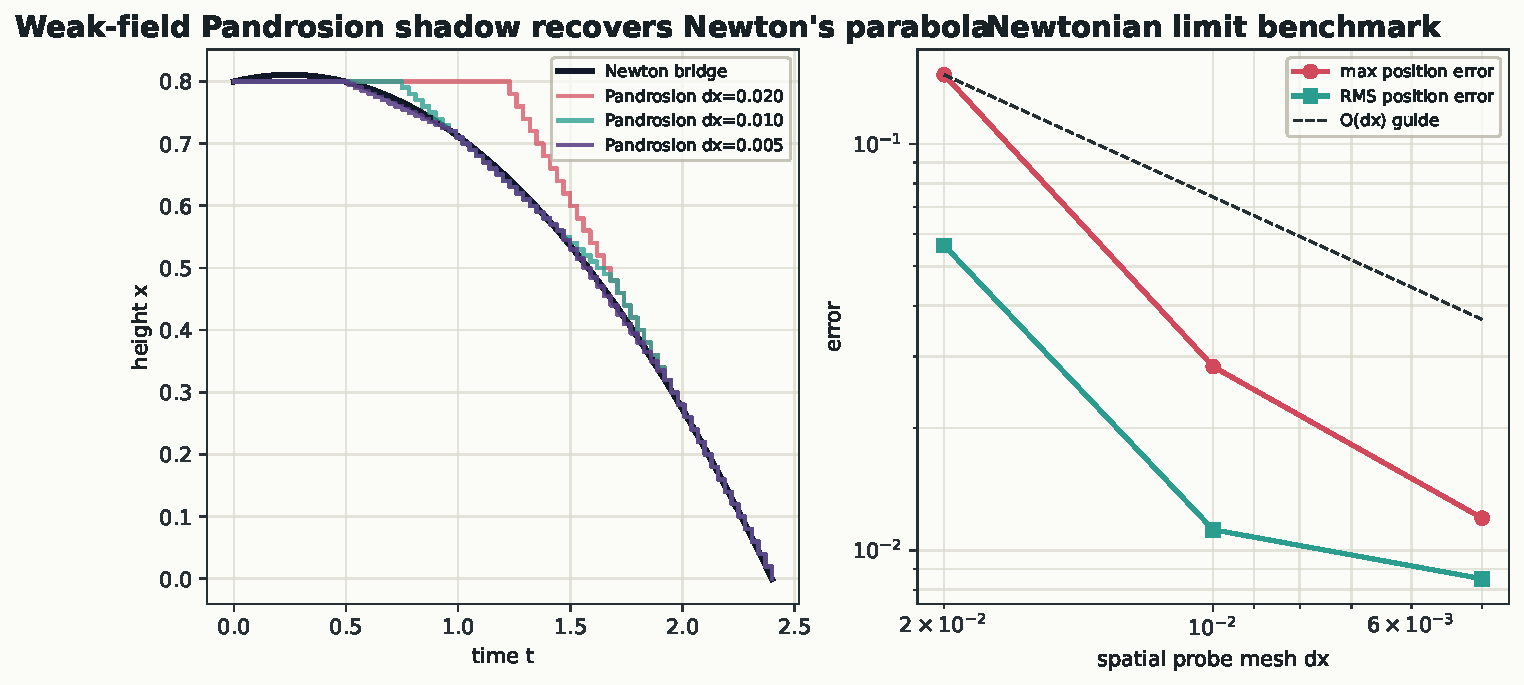
\includegraphics[width=0.96\linewidth]{028_newton_shadow_dp.pdf}
\caption{Newtonian shadow benchmark.  The finite weak-field Pandrosion score
selects a path converging to the constant-field Newtonian bridge.}
\label{fig:newton}
\end{figure}

The numerical test uses \(g=\NewtonGravity\), \(T=2.4\), \(x_0=0.8\), and
\(x_1=0\).  At the finest mesh \(\Delta x=\NewtonFineDx\), the maximum
position error is \(\NewtonFineMaxError\) and the RMS error is
\(\NewtonFineRmsError\).

\section{Benchmark 3: horizon-safe dynamic atlas}

The third test checks that a Pandrosion atlas distinguishes physics from bad
coordinates.  Consider radial Schwarzschild geometry with \(M=1\).  In
Schwarzschild coordinates,
\[
        f(r)=1-\frac{2M}{r},
        \qquad
        \dd s^2=-f(r)\dd t^2+f(r)^{-1}\dd r^2,
\]
so the coordinate description is singular at \(r=2M\).  In
Painleve--Gullstrand time \(T\),
\[
        \dd s^2
        =
        -f(r)\dd T^2
        +
        2\sqrt{\frac{2M}{r}}\,\dd T\,\dd r
        +
        \dd r^2,
\]
which is regular at the horizon.

For radial free fall from rest at infinity,
\[
        \frac{\dd r}{\dd T}=-\sqrt{\frac{2M}{r}},
        \qquad
        r(T)=
        \left(
        r_0^{3/2}-\frac32\sqrt{2M}\,T
        \right)^{2/3}.
\]
In the Painleve--Gullstrand chart this path has \(\dd\tau=\dd T\).  The
finite segment estimator therefore gives
\[
        \sum_k \tau_{h,\mathrm{PG}}=\HorizonPGTau,
        \qquad
        |T_{\mathrm{end}}-\sum_k\tau_{h,\mathrm{PG}}|
        =
        \HorizonPGTauError.
\]

\begin{definition}[Chart condition score]
For the horizon benchmark use the model costs
\[
        C_{\mathrm{Sch}}(r)=1+\frac{0.02}{|f(r)|^2},
        \qquad
        C_{\mathrm{PG}}(r)=1.32+0.08\left(\frac{2M}{r}\right)^2.
\]
The dynamic Pandrosion atlas selects the chart with smaller condition cost.
\end{definition}

\begin{figure}[htbp]
\centering
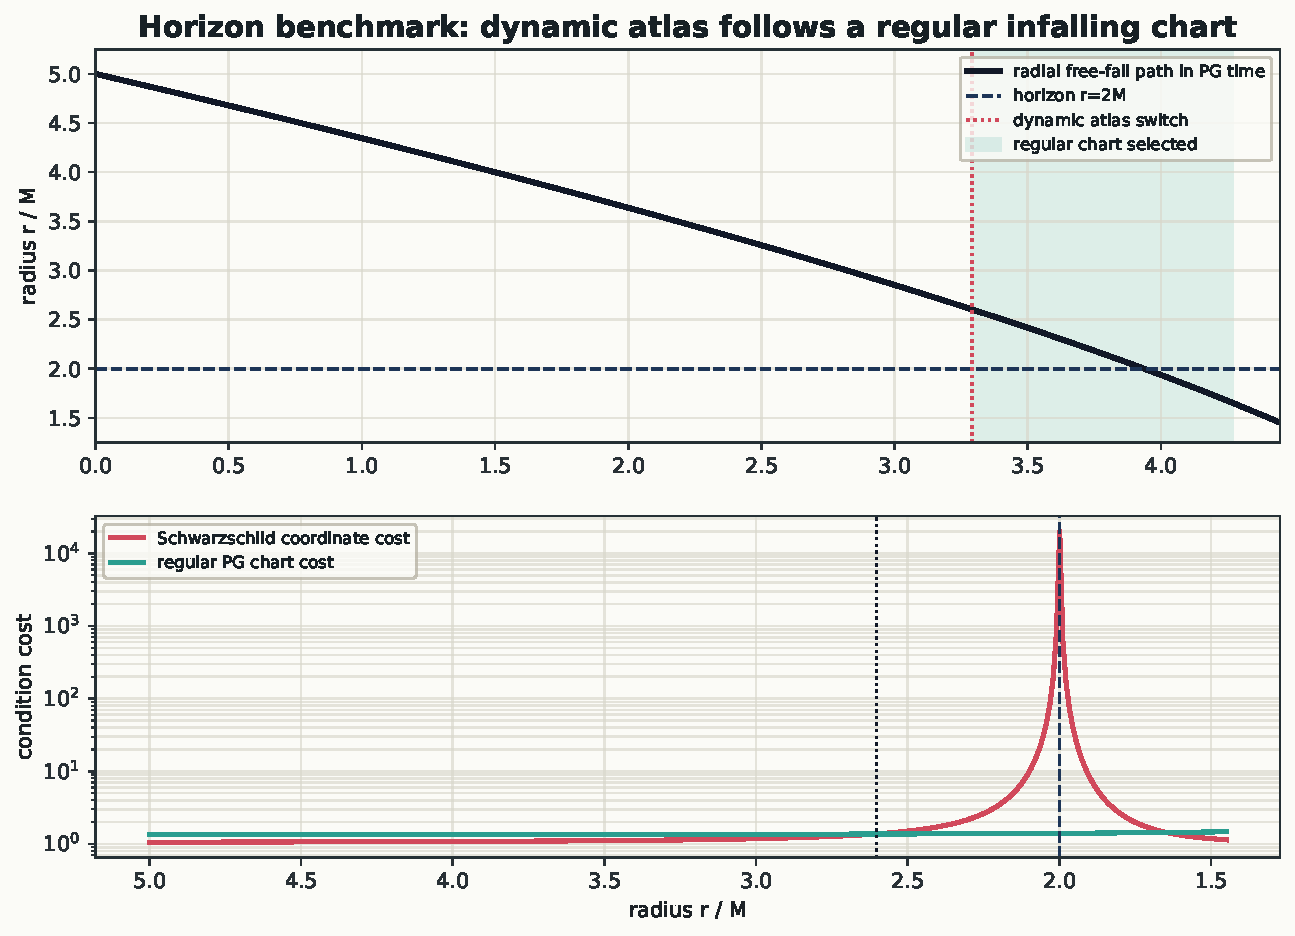
\includegraphics[width=0.94\linewidth]{028_horizon_atlas_benchmark.pdf}
\caption{Horizon atlas benchmark.  The physical infall path is regular, but
the Schwarzschild coordinate cost diverges near \(r=2M\).  The dynamic
Pandrosion atlas switches to the regular Painleve--Gullstrand chart before the
horizon.}
\label{fig:horizon}
\end{figure}

In the run shown in Figure~\ref{fig:horizon}, the atlas switches at
\[
        r\simeq \HorizonSwitchRadius M,
        \qquad
        T\simeq \HorizonSwitchTime.
\]
This is the numerical analog of the Riemann-chart logic in monomial
Pandrosion: when one coordinate representation becomes unstable, the method
changes chart while preserving the underlying invariant.

\section{Benchmark summary}

\begin{table}[htbp]
\centering
\renewcommand{\arraystretch}{1.18}
\begin{tabular}{p{0.24\linewidth}p{0.31\linewidth}p{0.35\linewidth}}
\toprule
Test & Classical invariant & Pandrosion result \\
\midrule
Minkowski & inertial line and proper time
& causal graph path error \(\MinkFinePathError\), proper-time gap
\(\MinkFineTauError\) at \(\Delta x=\MinkFineDx\) \\
Weak field & Newton equation \(x''=-g\)
& finite score recovers the parabolic bridge with RMS error
\(\NewtonFineRmsError\) at \(\Delta x=\NewtonFineDx\) \\
Horizon chart & regular infall across \(r=2M\)
& atlas switches to PG chart at \(r\simeq\HorizonSwitchRadius M\) and keeps
proper-time error \(\HorizonPGTauError\) \\
\bottomrule
\end{tabular}
\caption{The three validation layers for Pandrosion relativity.}
\label{tab:summary}
\end{table}

The results support the narrow claim of Paper 027.  Pandrosion is not replacing
relativity.  It gives a finite-probe calculus whose leading score reproduces
relativistic and Newtonian invariants when the graph and chart logic are
consistent.

\section{What remains to prove}

The benchmarks suggest four precise next targets:
\begin{enumerate}[label=(\roman*)]
\item prove convergence rates for the causal graph score with finite
tie-breakers and acceleration penalties;
\item extend the weak-field test to nonconstant potentials and compare with
standard symplectic variational integrators;
\item test horizon charting with full geodesic optimization rather than a
known analytic radial infall path;
\item combine finite holonomy from Paper 027 with stress-energy sampling to
test an Einstein-tensor balance on small lattices.
\end{enumerate}

\section{Conclusion}

Paper 028 gives the first computational validation layer for Pandrosion
relativity.  The method passes three sanity checks: it recovers inertial
motion in Minkowski space, recovers Newton's equation in the weak-field
slow-motion limit, and avoids a horizon coordinate singularity by dynamic
atlas switching.  The original contribution is not a new law of physics; it is
the Pandrosion protocol that treats these classical laws through causal
finite-slope probes and chart-invariant scoring.

\begin{thebibliography}{9}
\bibitem{wald}
R. M. Wald, \emph{General Relativity}, University of Chicago Press, 1984.

\bibitem{oneill}
B. O'Neill, \emph{Semi-Riemannian Geometry}, Academic Press, 1983.

\bibitem{regge}
T. Regge, \emph{General relativity without coordinates}, Nuovo Cimento 19,
558--571, 1961.

\bibitem{marsdenwest}
J. E. Marsden and M. West, \emph{Discrete mechanics and variational
integrators}, Acta Numerica 10, 357--514, 2001.

\bibitem{paper019}
I. Besevic, \emph{Discrete Geodesic Probe Convergence for Pandrosion},
manuscript, May 2026.

\bibitem{paper027}
I. Besevic, \emph{Pandrosion Relativity: Finite-slope causal probes, dynamic
atlases, and geodesic physical motion}, manuscript, May 2026.
\end{thebibliography}

\end{document}
